\documentclass[twocolumn]{scrartcl}
%\documentclass[twocolumn,12pt]{article}
%\documentclass{scrartcl}

\usepackage[utf8]{inputenc}
\usepackage[T1]{fontenc}
\usepackage{lmodern}
\usepackage[ngerman]{babel}
\usepackage{amsmath}

%\usepackage{makeidx}
%\makeindex

\usepackage{fancyvrb}
\usepackage{fvextra}

% \usepackage{palatino}
%
% \usepackage{newpxtext,newpxmath}
%
\usepackage[sc]{mathpazo} % or option osf
\usepackage{newpxmath}
\usepackage[output-decimal-marker={,}]{siunitx}

\usepackage[comma,authoryear]{natbib}
%\bibliographystyle{natdin}
%\bibliographystyle{apalike}
\bibliographystyle{apalike-german}

\usepackage{adjustbox}
\usepackage[a4paper, margin=1mm, includefoot, footskip=15pt]{geometry}
%\usepackage[a4paper, margin=20mm, includefoot, footskip=15pt]{geometry}
\usepackage{afterpage}

\usepackage{subcaption}
\usepackage[autostyle,german=guillemets]{csquotes}

\usepackage[pdftitle={Schnellwüchsige, geradschaftige Robinien}
, pdfauthor={Georg Kindermann}
, pdfsubject={Waldbau, Waldwachstum, Robinie, geradschaftig}
, pdfkeywords={Waldbau, Waldwachstum, Wald, Forst, Robinie, geradschaftig}
, pdflang={de-AT-1996}
, hidelinks
, pdfpagemode=None]{hyperref}

\nonfrenchspacing
\sloppy
\usepackage{breqn}
\usepackage{enumitem}
%\usepackage{rotating}
\usepackage{pdflscape}

\title{Schnellwüchsige, geradschaftige Robinien}
\author{Georg Kindermann}
%\date{22. Juli 2025}

\listfiles
\begin{document}

\twocolumn[
  \begin{@twocolumnfalse}
    \maketitle
    \begin{otherlanguage}{english}
    \begin{abstract}
      \begin{center}
        \textbf{Fast-growing, straight-trunked black locust}
      \end{center}
      The black locust (Robinia) copes relatively well with dry sites. However, many varieties develop trunks of inferior quality and are therefore mostly suitable only as firewood. Since the 1930s at the latest, black locusts have been selectively bred for straight growth, rapid development, and good drought resistance. Today, there are more than ten varieties that possess these traits. However, only a few of them are available in Austria. To gain practical experience and allow a comparative assessment of the new varieties, a small-scale trial was conducted in which three varieties purchased in Austria and five in Hungary were planted at three different sites.
    \end{abstract}
    \end{otherlanguage}
    \begin{abstract}
      Die Robinie kommt mit trockenen Standorten relativ gut zurecht.
      Viele Sorten entwickeln jedoch einen Stamm von minderer Qualität und eignen sich daher meist nur als Brennholz.
      Seit spätestens den 1930er--Jahren werden Robinien gezielt auf geraden Wuchs, schnelles Wachstum und gute Trockenresistenz gezüchtet.
      Heute existieren mehr als zehn Sorten, die diese Eigenschaften erfüllen.
      In Österreich sind jedoch nur wenige davon erhältlich.
      Um praktische Erfahrungen zu sammeln und einen vergleichenden Eindruck der neuen Sorten zu ermöglichen, wurden im Rahmen eines Kleinstversuchs drei in Österreich und fünf in Ungarn gekaufte Sorten an drei Standorten gepflanzt.
    \end{abstract}
  \end{@twocolumnfalse}
]

\tableofcontents

\section{Einleitung}

An bereits niederschlagslimitierten Standorten schränken zunehmende Trockenheit
und Wärme sowohl die Bandbreite wirtschaftlich vertretbarer waldbaulicher
Maßnahmen als auch die Auswahl geeigneter Baumarten zunehmend ein. Unter den
heimischen Hauptbaumarten kommen meist die Weiß-- (Pinus sylvestris) und
Schwarzkiefer (Pinus nigra) sowie verschiedene Eichenarten in Betracht. Die
Reihung der heimischen Eichen nach zunehmender Trockenresistenz erfolgt meist:
Stieleiche (Quercus robur), Traubeneiche (Quercus petraea), Zerreiche (Quercus
cerris), Flaumeiche (Quercus pubescens). Leider nimmt auch die Holzqualität nach
dieser Reihung ab. Das Holz der Zerreiche kann nicht zur Fassproduktion
verwendet werden, da es aufgrund ihrer weiten Poren nicht dicht ist und auch der
Splint ist breiter. Flaumeichen mit guter Qualität sind selten, wobei es in
letzter Zeit Züchtungen und Kreuzungen mit anderen Eichen gibt die sehr genügsam
bezüglich Niederschlagsmengen sind und eine gerade Schaftform bilden.

Solange es für einen Standort regionale Baumarten aus tieferen Lagen gibt,
scheint es, angesichts der Klimaerwärmung zweckmäßig, diese in höheren Lagen zu
verwenden. Befindet man sich jedoch in der tiefsten Höhenstufe, tendieren manche
dazu Baumarten aus südlichen bzw.\ äquatornäheren Regionen zu verwenden. Dort
mag zwar die Temperatur höher sein, Sonnenstrahlung und Tageslängen werden sich
hingegen meist unterscheiden. Auf demselben Breitengrad findet man höhere
Sommertemperaturen in kontinentaleren Regionen, was bei uns in Österreich in
Richtung Osten wäre.

Mit zunehmender Trockenheit wird die Verjüngung schwieriger, was eine
Verschiebung der Betriebsart vom Hochwald über Mittelwald hin zum Niederwald zur
Folge hat. Dieser Wechsel der Betriebsart geht Hand in Hand mit einer Förderung
von Baumarten mit gutem Ausschlagvermögen. Aus forstwirtschaftlicher Sicht ist
neben Stockausschlag die Fähigkeit zur Bildung von Wurzelbrut auf
verjüngungswidrigen Standorten zu begrüßen, da die Ausschläge nicht an einen
qualitätsmindernden Stock gebunden und daher meist gleichmäßiger auf der Fläche
verteilt sind. Während Stockausschlag nach etwa drei Umtrieben in der Regel
deutlich an Zuwachsleistung und Neuausschlagvermögen verliert, zeigt Wurzelbrut
diesen unerwünschten Effekt kaum bis gar nicht. Ausreichend Wurzelbrut bilden
von den heimischen Baumarten Aspe (Popukus tremula), Grauerle (Alnus incarna),
Ulme (Ulmus spp.), Feldahorn (Acer campestre), Kirsche (Prunus avium) sowie
Wildobst. Von den nicht heimischen bilden beispielsweise Robinie (Robinia
pseudoacacia) oder Götterbaum (Ailianthus altisima) reichlich Wurzelbrut.

Diese Eigenschaft ist aber auch ein Grund warum diesen Baumarten das Potential
eines invasiven Neophyten attestiert wird. Sie sind dadurch eher als andere
Baumarten in der Lage beispielsweise Trockenrasen zu besiedeln. Dabei wird man
die Frage stellen dürfen, wie diese Trockenrasengesellschaften entstanden sind.
Gelegentlich wird sich zeigen, dass sie in der Vergangenheit durch
(Brand\mbox{--)}Rodung eingeleitet wurden, ein Vorgang, der neuerdings, offenbar
in wörtlicher Anlehnung an den englischen Begriff deforestation, als
\enquote{Entwaldung} bezeichnet wird. Danach kam es zu Erosion,
Plaggenwirtschaft und Beweidung meist durch Schaf und Ziege. Nach Einstellung
der Bewirtschaftung ist eine natürliche Sukzession, zunächst über heimische
Sträucher wie Schlehe (Prunus spinosa), Weißdorn (Crataegus monogyna), Hundsrose
(Rosa canina), Kreuzdorn (Rhamnus cathartica), Liguster (Ligustrum vulgare),
Berberitze (Berberis vulgaris), Rote Heckenkirsche (Lonicera xylosteum),
Besenginster (Cytisus scoparius), Heidelbeere (Vaccinium myrtillus),
Kornelkirsche (Cornus mas) oder Roter Hartriegel (Cornus sanguinea) in Richtung
eines Waldes mit Traubeneiche (Quercus petraea), Stieleiche (Quercus robur),
Zerreiche (Quercus cerris), Flaumeiche (Quercus pubescens), Hainbuche (Carpinus
betulus), Feldahorn (Acer campestre), Birke (Betula pendula), Weißkiefer (Pinus
sylvestris), Schwarzkiefer (Pinus nigra) oder Winterlinde (Tilia cordata) nichts
Ungewöhnliches. Dies veranschaulicht eine Fläche auf der kleinen
Perchtoldsdorfer Heide, die 1940 als Naturdenkmal eingezäunt und seit dem so gut
wie nicht mehr beweidet, sondern der natürlichen Entwicklung überlassen wurde
\citep{rosenkranz1953heide}. Zu Beginn war man noch begeistert über die üppige
Blütenpracht der nun nicht mehr beweideten Fläche, aber bald schon begann die
Verbuschung. 1952 gab es dort einen Steppenbrand, wonach sich neben
Trockenrasenpflanzen auch Föhren einfanden \citep{rosenkranz1953heideBrand}. Ich
kenne diese Fläche seit den 1980er--Jahren, als sie bereits größtenteils zu
einem Wald aus Schwarzkiefern und Eichen geworden war.

Ein zusätzlicher Aspekt bei der Robinie ist ihre Symbiose mit
stickstofffixierenden Bakterien. Dadurch reichert sie den Boden mit Stickstoff
an, was meist die Wuchsleistung des Standorts erhöht. Dies schafft günstige
Bedingungen für die Etablierung weiterer Arten, die in der Folge die
konkurrenzschwachen Pflanzen der Trockenrasengesellschaft sukzessive verdrängen
können. Einheimische Arten wie Hornklee (Lotus corniculatus), Kleiner Wundklee
(Anthyllis vulneraria), Hufeisenklee (Hippocrepis comosa), Sichelklee (Medicago
falcata), Hopfenklee (Medicago lupulina) oder Wiesen--Platterbse (Lathyrus
pratensis) sind typische Begleitarten von Trockenrasen.
%und besitzen die Fähigkeit, Stickstoff zu fixieren.
Weiter heimische Leguminosen wie Besenginster (Cytisus scoparius),
Frühlings-Platterbse (Lathyrus vernus) oder auch die Esparsette (Onobrychis
viciifolia) treten eher im Zuge der natürlichen Sukzession auf und verdrängen
langfristig Trockenrasen--Gesellschaften. Sie alle können ebenso wie die
Robinie, Luftstickstoff im Boden fixieren.

\section{Gebietsfremde Baumart}

Auch wenn manche Trockenrasen keinen natürlichen Ursprung haben, wird ihre
Erhaltung, genauso wie die von Schottergruben, Ziegelteichen oder Steinbrüchen,
bei denen ihr anthropogener Ursprung für jeden offensichtlich ist, aufgrund
ihrer einzigartigen Standortseigenschaften, berechtigt sein. Es ist aus meiner
Sicht positiv zu bewerten, dass die geltenden Regelungen, zur Erhaltung
gefährdeter Lebensräume, die forstliche Nutzung nicht-heimischer Baumarten nicht
grundsätzlich ausschließen. Nur bei einer Baumart, dem Götterbaum (Ailanthus
altissima), ist dies in Österreich zurzeit nicht der Fall. Der Götterbaum wurde
in \cite{eu2019verordnungListeInvasiverArten} mit Bezug auf
\cite{eu2014verordnungInvasiverArten} aufgelistet und wurde in der Folge aus der
im Anhang des Forstgesetz 1975 angeführten Liste der Holzgewächse entfernt und
kann somit rechtlich keinen Wald bilden. Diese Liste soll mindestens alle sechs
Jahre überprüft und aktualisiert werden. Aufgelistete Arten müssen: gebietsfremd
sein; sich ausbreiten können; nachteilige Auswirkungen auf Biodiversität,
Ökosystemdienstleistungen, menschliche Gesundheit oder die Wirtschaft haben; es
musse nachgewiesen sein, dass zur Verhütung ihrer Einbringung, Etablierung oder
Ausbreitung konzertierte Maßnahmen erforderlich sind; es muss wahrscheinlich
sein, dass die nachteiligen Auswirkungen tatsächlich verhindert, minimiert oder
abgeschwächt werden können. Aufgelistete Arten dürfen nicht vorsätzlich in das
Gebiet der Union verbracht, gehalten oder gezüchtet werden: in die, aus der und
innerhalb der Union befördert werden; in Verkehr gebracht oder in die Umwelt
freigesetzt werden; verwendet oder getauscht werden. Zusätzlich werden
angemessene Managementmaßnahmen erarbeitet, welche die Auswirkungen auf die
Biodiversität und die damit verbundenen Ökosystemdienstleistungen, sowie
gegebenenfalls auf die menschliche Gesundheit oder die Wirtschaft durch diese
Arten minimieren, sowie beeinträchtigt, geschädigt oder zerstörte Ökosysteme
wiederherzustellen. Davon ausgenommen sind Arten in den Regionen in äußerster
Randlage von unionsweiter Bedeutung sind, wobei für diese Regionen diese Arten
aufgelistet werden müssen. Ausnahmen können für die Einrichtungen, die
Durchführung von Forschung und Ex-situ-Erhaltung genehmigt werden und in
Ausnahmefällen können Zulassungen erteilt werden. Zusätzlich können
Mitgliedstaaten Arten, die für sie von Bedeutung sind, auflisten und abweichende
Maßnahmen treffen. Gesetzlich vorgeschriebene Maßnahmen können vom
Grundeigentümer verlangen, dass er auf eigene Kosten, Arten zu bekämpfen, die er
nie ausgebracht hat, wie dies bei Ragweed im Burgenland der Fall ist
\citep{burgenland2021ragweed}.
%Nach
%\cite{huber2025goetterbaum} sind die Holzeigenschaften des
%Götterbaumes vergleichbar mit denen der Esche, welche durch das
%Eschentriebsterben stark dezimiert wurde. Allerdings war es den
%Autoren, offensichtlich durch die Einstufung als invasiver Neophyt,
%kaum möglich qualitativ hochwertiges Holz aus Wäldern zu
%bekommen. Auch wenn sich der Götterbaum invasiv verhält, stellte
%\cite{hasenauer2014waldbauNewsletter} bei einer künstliche Aufforstung
%Ausfälle zwischen 51--100\,\%, im zweiten Herbst nach der Pflanzung,
%fest.

Umgekehrt gibt es auch die Möglichkeit das Baumarten gesetzlich
geschützt werden, wie dies bei der Eibe (Taxus baccata) in
Niederösterreich der Fall ist
\citep{niederoesterreich2000Naturschutzgesetz,niederoesterreich2005artenschutzverordnung}. Die
Eibe wird dort als pflückgefährdet eingestuft. Eine zeitgemäße und
nachhaltige gewerbliche, land- und forstwirtschaftliche Nutzung wird
nicht untersagt. Dennoch entsteht Verunsicherung und kann dazu
führen, dass der eine oder andere deswegen vor einer forstliche
Anpflanzung von Eiben zurückschreckt.

Gesetzliche Rahmenbedingungen können sich ändern. Wer sein Risiko von diesem Gesichtspunkt aus minimieren
möchte, sollte ausgewählte Sorten, eher nur dort einbringen, wo bereits Robinien sind.
Andererseits wird man bei einer massiven Standortsveränderung, wie dies die bereits erfolgte
und in Zukunft zu erwartende Temperaturerhöhung darstellt, mit der Etablierung gebietsfremder Arten rechnen müssen.

Nicht nur eine Standortsveränderung kann eine im Wald stockende Art
bedrohen, sondern auch Gesetzliche vorgaben. Für eine Waldbauliche
Planung und Entscheidungsfindung wäre es zweckmäßig Baumartenlisten zu
haben, bei denen Gesetzlich garantiert wird, dass deren Forstliche
Nutzung bis zur Hiebsreife möglich ist.
Sollte eine Bekämpfung erforderlich werden, sollte diese, ebenso wie eine
gegebenenfalls notwendige Verjüngung mit alternativen Baumarten, unterstützt werden.

\section{Veränderung des Standorts}

In \cite{oebf2019aliensAusDemGarten} findet sich: \enquote{Auch wenn die
Robinie entfernt wird, hat sie den Boden mit Stickstoff und giftigen
Ausscheidungen aus Wurzeln und Laub angereichert und die Pflanzenwelt
am Standort dauerhaft verändert. Von Wildtieren wird sie nicht
verbissen (dornig und giftig). \dots Unterdrückt nahezu jede andere
Pflanze und ist daher für die Gartengestaltung wenig
geeignet. Aufgrund zahlreicher Ausläufer schwer zu bekämpfen. Vorsicht
vor Verletzungen mit den giftigen Dornen!}. Leider gibt es in
der Broschüre keine Literaturangaben um die Quelle diese Aussage
zu verifizieren. Meiner Ansicht nach trägt sie dazu bei, dass die falsche
Meinung entsteht, die Robinie würde den Boden vergiften und damit den Wald zerstören.

Robinien können Luftstickstoff fixieren.
\cite{boring1984robinieN} berichten von 30\,kgN/ha/Jahr bei einem
vierjährigen Robinienbestand, \cite{noh2009robinieN} beobachteten
Fixierungsraten von 23--112\,kgN/ha/Jahr und \cite{danso1995robinieN}
von 220\,kgN/ha/Jahr in Robinienbeständen.

Unter den Heimischen Baumarten können Erlen Stickstoff fixieren. Dort
wird diese Eigenschaft mit Bodenverbesserung in Verbindung
gebracht. \enquote{Grundlage für die immer wieder betonte bodenverbessernde
Wirkung der Grauerle bildet ihre Fähigkeit zur Bindung von
Luftstickstoff mittels einer Actinorhiza}
\citep{schuett2014alnusIncarna}. \cite{schuett2014alnusIncarna} geben
auch einen aus der Literatur gesammelten Überblick der
Stickstoffixierungsraten von Grauerle mit 43--72\,kgN/ha/Jahr.

Leguminosen werden auch in der Landwirtschaft verwendet.
\cite{kolbe2008stickstoff} gibt Stickstoffbindungsmengen von
105--309\,kgN/ha durch Leguminosen im Ökolandbau an.

Der Düngemittel Reinnährstoffabsatz in Österreich liegt in Österreich
ca.\ bei 100\,000 t/N/Jahr \citep{ama2024duengemittel}. Laut Statistik
Austria wurden im Jahr 2020 1\,322\,900\,ha als Ackerland und
insgesamt 2\,602\,700\,ha landwirtschaftlich genutzt. Daraus errechnet
sich, wenn der abgesetzte N-Dünger nur auf Ackerland ausgebracht wurde
75\,kgN/ha bzw.\ 38\,kgN/ha, wenn die gesamte landwirtschaftlich
genutzt Fläche angesetzt wird.

Nach \cite{uba1998deposition} kann es bei der nassen Deposition von
Gesamtstickstoff zu Einträgen bis über 20\,kg/ha und Jahr kommen. Auch
\cite{raspe2018stickstoff} berichten von N-Einträgen über
20\,kg/ha/Jahr, welchen Austrägen von 6\,kg/ha/Jahr gegenüber
stehen. In Holz und Rinde werden je nach Baumart und Standort zwischen
4\,kg/ha/Jahr (Kiefer) und 16\,kg/ha/Jahr (Eiche) festgelegt und bei
einer anschließenden Ernte entzogen. Die gesamte Stickstoffaufnahme
von Bäumen ist deutlich höher und der mit dem Streufall rückgeführte
Stickstoff liegt bei 50\,kg/ha/Jahr. \cite{raspe2018stickstoff}
berichten von einer mittleren Stickstoffanreicherung von
ca.\ 6\,kg/ha/Jahr in den letzten 25~Jahren.
\cite{emberger1965stickstoff} fanden in Waldböden bis 1\,m Tiefe
Stickstoffvorräten zwischen 1905\,kg/ha und 15\,929\,kg/ha.

Stickstofffixierung durch Bäume in Wäldern ist selten anzutreffen.
Die Deposition kompensiert bzw.\ übersteigt leicht die Austräge bei
der Ernte.  Bei stickstoffgesättigten Böden ist damit zu rechnen, dass
es zu Auswaschungen kommt, was insbesondere in Quellschutzgebieten zu
vermeiden ist. An Standorten, an denen der Zuwachs der Bäume durch
Stickstoffgaben gesteigert werden kann, was beispielsweise in ehemals
streugenutzten Wäldern der Fall sein könnte, sollten
stickstofffixierende Pflanzen in der Regel willkommen sein. So
empfiehlt beispielsweise \cite{wiedemann1951ertragskunde} den Anbau
von Dauerlupine, um den Standort zu verbessern und die Wuchsleistung zu
steigern. Die Menge an Stickstoff, die die Robinie fixiert, entspricht
in ihrer Größenordnung etwa der von anderen Leguminosen wie Lupine
oder Klee, welche im Ökolandbau eingesetzt werden.

Die Veränderungen der Artenzusammensetzung unter Robinien wird eher durch
Veränderungen der Bodennährstoffverfügbarkeit und Lichtbedingungen
verursacht, als durch Allelopathie \citep{vitkova2017robinie}. Nach
\cite{mueller1991robinie} ist in den ersten Jahren nach Einbringung
der Robinie mit vorübergehend verstärktem Entzug der Hauptnährstoffe
Stickstoff, Phosphor und Kali infolge Nährstoffaufnahme des intensiven
Robinienwurzelsytems zu rechnen. Diese vorübergehende Festlegung von
Nährstoffen hat der Robinie den Ruf als \enquote{Nährstoffräuber}
eingetragen. Unter dem Einfluss der Robinie entwickelt sich eine
Verjüngungshemmende Ruderalflora (siehe Abb.~\ref{fig:glaswein}).

In den Untersuchungen von
\citet[S.~150--160]{scamoni1952robinieWurzeln} wird das Wachstum der
Wurzeln von benachbarten Ahornbäumen als auch benachbarter Robinien
durch Wurzeln anderer Robinien nicht gestört. Hingegen meiden nach
\citet[S.~53]{kolesnikov1971wurzeln} Wurzeln von Apfelbäumen den
Wurzelbereich anderer Apfelbäume, breiten sich jedoch zwanglos
zwischen Wurzeln von Kirsche und Marille aus.

Nach \cite{hanzelka2015robinie} sind in Mitteleuropa Robinienbestände
im gesamten Wachstumszeitraum lichter im Vergleich zu einheimischen
Wäldern und sowohl die Strauch-- als auch die Kräutschicht sind daher
dichter. Die Beschattung in Robinienbeständen lag bei 57\,\% im
Vergleich zu 72\,\% in einem einheimischen Eichenwald, die
Strauchbedeckung lag bei 57\,\% im Vergleich zu 11\,\% und die
Krautschicht bei 53\,\% im Vergleich zu 5\,\%.

Nach \cite{vitkova2017robinie} ist die Belaubungszeit der Robinie
relativ kurz. Die Blätter erscheinen spät im Frühjahr (Mai) und
beginnen früh zu fallen, normalerweise während der Sommertrockenheit
(August). Die hohe Lichtversorgung ermöglicht es auch lichtbedürftigen
Arten, Frühjahrsgeophyten oder einer dichten Strauchschicht, zu
überleben. Dies dichte Kraut-- und Schrauchvegetation ist jedoch
gleichzeitig ungünstig für die Verjüngung von schattenintoleranten
einheimischen Baumarten sowie auch für die Robinie selbst. Für
Pionierpflanzen ist es typisch, dass sie als Erstbesiedler einen
Standort für nachfolgende Pflanzen vorbereiten, von diesen aber
schließlich selbst verdrängt werden.

\citet[p.\,467, 586]{ashton2018silviculture} beschreibt ein
Agroforst-Weidewirtschaftssystem (silvopastoral system) wobei die
Robinie aufgrund ihrer Stickstoffbindungskapazität und ihres lichten
Blätterdaches das Wachstum der darunter liegenden Gräser fördert.

\begin{figure}[htbp]
  \centering
  \includegraphics[width=.9\linewidth]{./bild/GlasweinRobinie2023a}
  \caption{Robinienversuchsfläche in Glaswein mit üppigem Unterwuchs}
  \label{fig:glaswein}
\end{figure}

Einmal etablierte Robinien sind aufgrund ihrer Ausschlagfähigkeit
bzw.\ Wurzebrut, insbesondere auf unbewirtschafteten Trockenrasen, aber
auch in lichten Wäldern, schwer wieder loszuwerden. Da sie zu den
Lichtbaumarten mit Pionierkarakter zählt, wird ihre Verjüngung durch
dichten Unterwuchs oder Schattbaumarten stark
eingeschränkt. Schalgflächen kann sie rasch wiederbestocken, ist aber
aufgrund ihrer lichtdurchlässigen Krone kaum in der Lage andere
Baumarten auszudunkeln.

\cite{jung2010robinie} beschreibt, dass die Japanische Walnuss (Juglans
ailanthifolia Carr.) allelopathische Aktivität gegenüber der Robinie
zeigt. Die Wurzeln des Baumes enthalten Juglon, welches das Wachstum
von Robiniensämlingen deutlich hemmte.

Robinien sind für Pferde giftig \citep{grosche2008robiniePferd}. Sie
wird aber von Hasen und Mäusen geschält bzw.\ deren Wurzeln gefressen,
was Aufforstungen auf Grasland erschwert, und vom Reh verbissen
\citep{barta2023robinieReh}. Nach \cite{berner2018robinie} werden
Robinien von Kühen nicht verbissen. Robinienblätter eignen sich als
Futter für Schafe \citep{ganai2009robnieSchaf}, Ziegen
\citep{papachristou1999robinieZiege} oder Hasen
\citep{singh2010robnieHasennahrung} wobei sie Immunfunktionen bei
Hasen verbessern \citep{yang2017robinieHasen}.
Zusätzlich spenden sie den Tieren Schatten.
Insbesondere in trockenen Regionen stehen sie jedoch mit anderen Pflanzen in Konkurrenz um Wasser \citep{halasz2021robinieAlsTierutter}.

\section{Geschichte}

\subsection{Bis zur Eiszeit}

Im Oligozän wurden Ablagerungen von zwei Robinienarten in Europa nachgewiesen.
Im Miozän wurden hingegen mehr als ein Dutzend Ablagerungen als Robinienart
identifiziert. Eine davon aus dem späten Miozän ähnelt der heutigen Robinie
Nordamerikas so stark, dass ihr Beschreiber geneigt war, beide als identisch
anzusehen. Diese Form war auch während des Pliozäns im europäischen Raum
verbreitet. Gleichzeitig war an der Mittelmeerküste Südeuropas eine zweite
Robinienart verbreitet. Es gibt keinen Hinweis, dass diese Robinienarten die
erste Eiszeit in Europa überlebt haben \citep{berry1918robinie}. Ihr
nacheiszeitliches natürliches Verbreitungsgebiet befindet sich im mittleren
östlichen Nordamerika (Abb.~\ref{fig:verbreitungNatuerlich}). Wien ist vom
Temperaturgang einzelnen Herkünften des natürlichen Verbreitungsgebietes
ähnlich, die Niederschlagsmenge ist in Wien jedoch deutlich geringer
(Abb.~\ref{fig:wetter}). Auch wenn der mittlere Monatsniederschlag deutlich
höher ist, können dennoch längere Perioden ohne Niederschlag, insbesondere auf
Böden mit geringer Wasserspeicherfähigkeit, auch in diesen Regionen
Trockenstress verursachen.

\begin{figure}[htbp]
  \centering
  \includegraphics[width=.9\linewidth]{./bild/map4}
  \caption{Natürliches Verbreitungsgebiet der Robinie nach \cite{little1971treeAtlas} sowie einzelne Herkünfte}
  \footnotesize{H\dots Harrisburg (Beste Herkunft nach \cite{cobbett1825woodlands}),
    S\dots Long Island (Erstbeschreibung Schifsmastrobinie \cite{raber1936shipmast}),
    X\dots Elkins (Beste Herkunft nach \cite{hopp1941robinie}) sowie Bartow und Thornwood -- Allegheny und Algonquin,
    A\dots Appalachia}
  \label{fig:verbreitungNatuerlich}
\end{figure}

\begin{figure}[htbp]
  \centering
  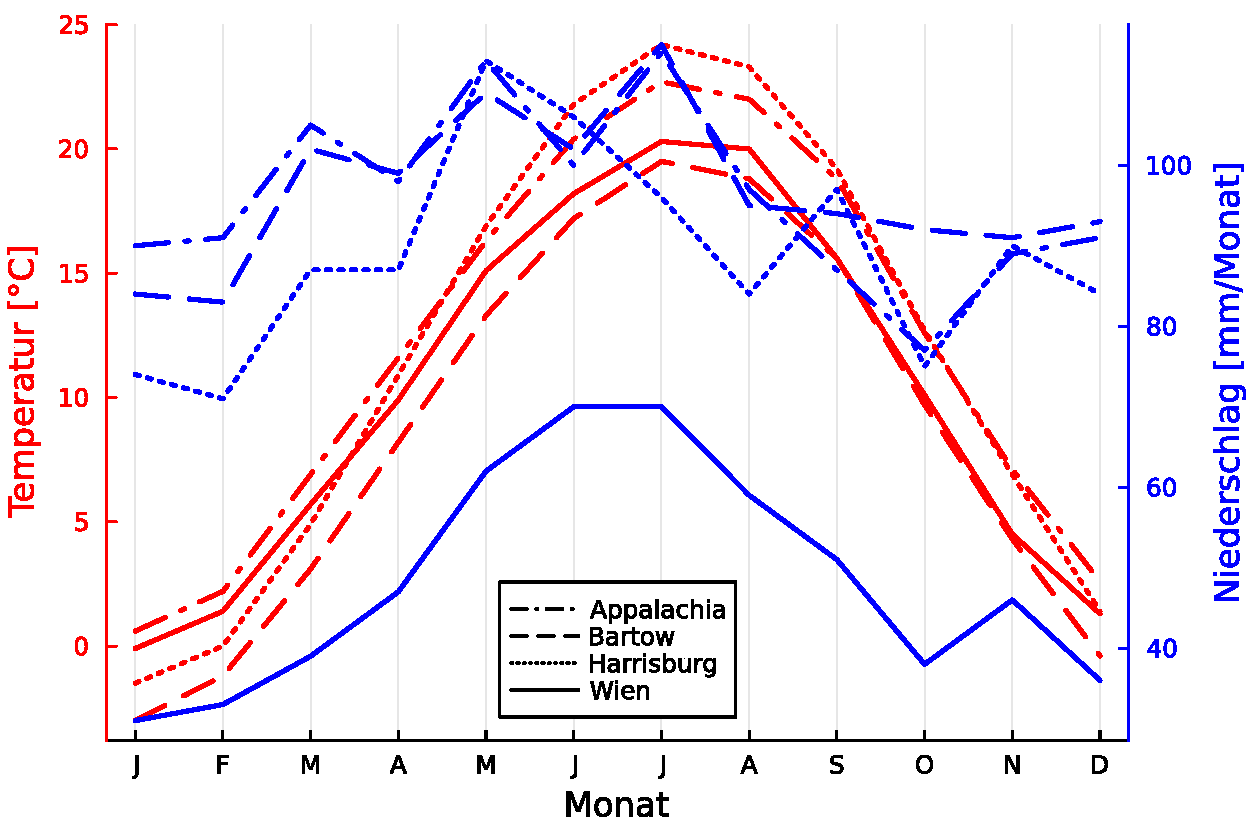
\includegraphics[width=.9\linewidth]{./bild/wetter}
  \caption{Temperatur und Niederschlag dreier Herkünfte sowie von Wien für den
  Zeitraum 1970--2000 abgefraht aus globalen Karten von \cite{worldclim2017}}
  \label{fig:wetter}
\end{figure}

\subsection{Erste schriftliche Erwähnungen}

Eine der ersten, wenn nicht sogar die erste, schriftliche Erwähnung
der Robinie (Locust), oder einer Baumart, die ihr ähnlich ist, stammt von
\cite{strachey1610-1612historie}: \enquote{The bowes are of some young
plant, eyther of the \emph{locust-tree} or of weech, \dots} (Die
Bögen bestehen aus einer jungen Pflanze, entweder aus dem Locust--Baum oder
der weech (witch-hazel -- virginischen Zaubernuss Hamamelis virginiana),
\dots) \enquote{By the dwellings of the salvages are bay-trees, wild
roses, and a kind of low tree, which bears a cod like to the peas, but
nothing so big: we take yt to be \emph{locust}.} (Bei den
Behausungen der Ureinwohner stehen Lorbeerbäume, wilde Rosen und eine
Art niedriger Baum, der eine Schote trägt, ähnlich den Erbsen, aber
nicht so groß; für uns sehen sie wie \enquote{Johannisbrotbäume} aus.)

Sie wurde Anfang des 17.~Jahrhunderts nach Europa gebracht und ist
dort mittlerweile weit verbreitet. Jedoch ist derzeit nicht bekannt,
wie und wann genau dies war. Nach derzeitigem Wissensstand wurde sie
erstmals 1634 von John Tradescant dem Älteren in England unter dem
Nahmen \emph{Locusta virginiana arbor} angeführt
\citep[S.~339]{gunther1922botanists}. John Tradescant
der Jüngere brachte von einer Reise nach Virginia mehrere Pflanzen mit
und könnte der erste gewesen sein, der Robiniensamen nach Europa
gebracht hat. Tradescant der Ältere war in Kontakt mit Vespasien
Robin und über diese Verbindung dürften Robiniensamen nach Paris
gekommen sein \citep{bouteiller2019robinie}.

\citet[S.~171--173]{cornuti1635robinie} beschreibt eine der Robinie
ähnliche Pflanze und gibt ihr den Namen \emph{Acacia Americana
Robini}. In der Beschreibung steht: \enquote{Succedunt semina Lenticulae
similia, quae singula singulis nucleis duris admodum, \& ex omni parte
echinatis clauduntur.} (Die linsenähnlichen Samen sind einzlen in
einzelnen Kapseln eingeschlossen, die sehr hart und auf allen Seiten
stachelig sind.) Die Robinie hat keine Samen die einzeln in einzelnen
stacheligen Kapseln sind.

\citet[S.~28]{deLaBrosse1636robinie} führt eine \emph{Acatia Indica}
an, die angeblich von Vespasien Robin gepflanzt wurde und heute noch
in Paris wächst.

\citet[S.~370]{gunther1922botanists} gibt in einer Liste Samen, die
von Virginia am 18~März 1636 die anscheinend Parkinson von Herrn
Morrice erhalten hat den Eintrag: \enquote{A yellow wood called
\emph{Locust} long flat blackish browne pods, black round flatt seede
kidney like.} (Ein gelbes Holz namens Locust mit langen, flachen,
schwärzlich-braunen Schoten und schwarzen, runden, flachen,
nierenförmigen Samen.), an.

\citet[S.~1550]{parkinson1640theatrumBotanicum} beschreibt die von
\cite{cornuti1635robinie} beschriebene \emph{Acacia Americana Robini}
und gibt ihr den Namen \emph{Pseudoacacia Americana Robini} um diese
von der Robinie, die er \emph{Arbor siliquosa Virginensis spinosa,
Locus nostratibus dicta, Virgin Locus tree} nennt, zu
unterscheiden. Er schreibt: \enquote{A very like tree hereunto hath beene sent and brought us out of \emph{Virginia}, growing to be a very great tree, and of an exceeding height with Masters \emph{Tradescant}, \dots}
(Ein sehr ähnlicher Baum ist uns aus Virginia gesandt und gebracht worden, der zu einem sehr großen Baum mit außergewöhnlicher Höhe heranwächst, bei Meister Tradescant.),
\enquote{We have not seene the tree to bear any flowers with us as yet nor fruite, but the cods that came to us, were small, long, and somewhat flat \dots, containing small grayish flat and round seede.}
(Wir haben den Baum bei uns bisher weder Blüten noch Früchte tragen sehen, aber die Schoten, die zu uns gelangten, waren klein, lang und etwas flach, \dots enthielten kleine, gräuliche, flache und runde Samen.),
\enquote{\dots is called Locus by our Nation resident in Virginia.}
(\dots Wird von unseren in Virginia ansässigen Landsleuten Locus genannt.).

1696 wurde die erste Robinie in Wien gepflanzt
\citep[S.~147]{loudon1838arboretum1}.

\citet[S.~3]{vadas1911robinie} schließt aus alten Bäumen, das
die Robinie erstmals um 1710--1720 in Ungarn gepflanzt wurde, was von
\citet[S.~179]{ernyey1926robinie} angezweifelt wird. Er führt an, dass
János György (Johann Georg Heinrich) Kramer 1735 die Robinie zur
Aufforstung in Ungarn erstmals empfiehlt.

In der Zwischenzeit hat
sich die Robinie in Europa und auch global verbreitet
(Abb.~\ref{fig:verbreitungGlob}, \ref{fig:verbreitungEuJetzt}). Laut
\cite{bouteiller2019robinie} stammen die Robinien in Europa von vier
Populationen aus Nordamerika ab und weisen eine geringe genetische
Vielfalt auf. Die ersten Exemplare wurden im frühen 17.\ Jahrhundert
vermutlich aus Virginia eingeführt, während des 17.\ und
18.\ Jahrhunderts kamen weitere aus Pennsylvania und West Virginia
hinzu. Diese scheinen die Mutterpflanzen der meisten, heute in Europa
vorkommenden, Robinien zu sein.

\begin{figure}[htbp]
  \centering
  \includegraphics[width=.9\linewidth]{./bild/verbreitungRobGlob}
  \caption{Verbreitung der 385\,746 Beobachtugnen von Robinie nach \cite{gbifRob}}
  \label{fig:verbreitungGlob}
\end{figure}

\begin{figure}[htbp]
  \centering
  \includegraphics[width=.9\linewidth]{./bild/verbreitungEuropa}
  \caption{Derzeitige Verbreitung der Robinie in der Europäischen Union nach \cite{jrc2016treeAtlas}}
  \label{fig:verbreitungEuJetzt}
\end{figure}

Abbildung~\ref{fig:verbreitungEuPot} zeigt die derzeitige standörtliche Eignung
für Robinien. So gut wie alle Tieflagen in Österreich sind demnach tauglich, was
auch durch registrierte Beobachtungen von Robinie belegt wird
(Abb.~\ref{fig:verbreitungEur}). Für eine waldbauliche Planung ist jedoch
besonders in Zeiten des Klimawandels nicht nur eine derzeitige, sondern auch
eine zukünftige Standortseignung zu berücksichtigen. In
Abbildung~\ref{fig:verbreitungEuPotZukunft} ist die erwartete Standortseignung
der Robinie beim Klimawandelszenarion mit sehr starker Temeraturerhöhung
(RCP~8.5) für das Jahr 2095 dargestellt. Demnach sollten die meisten derzeit in
Österreich für Robinie tauglichen Standorte auch in Zukunft tauglich bleiben.
Selbstverständlich sind solle Schätzungen mit Unsicherheiten verbunden, jedoch
sollte die Gefahr, dass ein Standort seine Tauglichkeit im Lauf der Zeit
verliert, bei Baumarten die relativ kurze Umtriebszeiten erlauben, geringer
sein, als bei solchen mit sehr langen. Die meisten Baumarten sind laut
Forstgesetz erst ab 60~Jahren hiebsreif. Die Robinie ist in der Verordnung für
Raschwüchsige Baumarten aufgenommen, wo die Obergrenze ihrer Hibsunreife mit
10~Jahren festgelegt ist. Umtriebszeiten von 15--30~Jahren sind mit Robinie auf
durchschnittlichen Standorten möglich und lassen sich bei Bedarf durchaus auch
auf 100~Jahre ausdehnen.

\begin{figure}[htbp]
  \centering
  \includegraphics[width=.9\linewidth]{./bild/potentialEuropaAtlas}
  \caption{Derzeitige standörtliche Tauglichkeit für die Robinie in der Europäischen Union nach \cite{jrc2016treeAtlas}}
  \label{fig:verbreitungEuPot}
\end{figure}

\begin{figure}[htbp]
  \centering
  \includegraphics[width=.9\linewidth]{./bild/verbreitungRobEur}
  \caption{Lage der Beobachtungen von Robinie in Europa nach \cite{gbifRob}}
  \label{fig:verbreitungEur}
\end{figure}

\begin{figure}[htbp]
  \centering
  \includegraphics[width=.9\linewidth]{./bild/potentialEuropaZukunft85}
  \caption{Potentielle standörtliche Tauglichkeit der Robinie im Jahr 2095 bei einer Klimaentwicklung nach RCP8.5 nach \cite{mauri2022baumartenZukunft}}
  \label{fig:verbreitungEuPotZukunft}
\end{figure}

\subsection{Selektion und Züchtung}

Auch wenn die genetische Bandbreite in Europa eingeschränkt sein soll,
gibt es dennoch Variationen und so berichtet
\citet[S.~259--260]{Michaux1813arbres} von einer Dornenlosen Robinie
(Robinia pseudoacacia spectabilis) welche von M.~Descemet aus
Saint-Denis um 1803--1805 entdeckt wurde und sich besonders gut für
Niederwälder eignen. Zusätzlich soll sie auch noch schneller als die
anderen wachsen. Auch wurde beobachtet, dass aus Samen von dieser
Pflanze gezogene Nachkommen wieder bedornt waren, aber
\cite{Michaux1813arbres} vermutet, dass die Samen von diesen bedornten
Nachkommen dornenlose Nachkommen hervorbringen
werden. \citet[S.~173]{quatrefages1861robinie} beschreibt, dass diese
Varietät vegetativ vermehrt wurde und mittlerweile auf der ganzen Welt
zu finden sei.

Robinie lässt sich vegetativ relativ einfach über Wurzelschnittlinge
vermehren. Da die vegetative Vermehrung schon seit langer Zeit
praktiziert wird, kann es vorkommen, dass später gemachte Selektionen,
von verschiedenen Orten, genetisch ident sind
\citep{liesebach2012robinie}. Der Duchmesser von Wurzelschnittlingen sollte zwischen 1/4
und 1 Zoll (0,6--2,5\,cm) stark sein und Längen von ca. 3--5~Zoll
(8--13\,cm) haben. Die Ausbeute von jungen Bäumen, vorzüglich jene die
in der Baumschule zum Verpflanzen ausgegraben wurden, ist deutlich
besser als jene von alten (bis zu 80\,\% der Schnittlinge von Jungpflanzen treiben aus).
Bis zu 50\,\% des Schnittlinge von älteren Bäumen trieben aus, wenn diese
Wuzelstärken zwischen 2--4\,cm hatten.
Der Wuzelschnitt und die Pflanzung sollen vor dem
Austrieb im Frühling erfolgen. Wurzeln müssen vor dem Austrocknen und
vor Frost geschützt werden. Waagrecht gepflanzte Wurzeln hatten eine
höhere Ausbeute gegenüber lotrecht gepflanzten, was eventuell durch
kopfüber Ausrichtungen bei den Lootrechten bedingt sein kann. Eine
lotrechte Wurzelausrichtung führt zu besseren Jungpflanzen, erfordert
aber möglicherweise eine Markierung der richtigen
Ausrichtung. Andererseits verlaufen viele Wurzeln in ihrer natürlichen
Lage waagrecht, insbesondere diejenigen, die im Wald Wurzelbrut bilden.
Leichte Böden wie sandiger Lehm
eignen sich für die Anzucht wobei in den ersten Wochen eventuell
gegossen werden sollte. Sprossrückschnitte während des Wachstums sind
schlecht. Stecklinge sowohl aus unverholzten als auch verholzten
Jungtrieben bekommen nur ganz selten Wurzeln
\citep{swingle1937robinie}.

\cite{keresztesi1983robinie} unterteilt ausgewählte Robiniensorten in
die Klassen: Schnittholz (bessere Standorte); Pfähle und Posten
(mittlere Standorte); Imkerei und dekorative Bepflanzung. Manche
Sorten sollen sowohl forstlich als auch zur Honigproduktion geeignet
sein. Für die Honigernte interessant sind frühblüher (var.\ praecox),
spätblüher (var.\ galiana) und dauer-- bzw. öftersblüher
(var. semperflorens Carrière). \cite[S.~80]{crane1985honig} gibt ein
Honigpotential von 48--1600\,kg/ha für Robinie an. Zum Vergleich werden
20--42\,kg/ha beim Apfel, 100--200\,kg/ha bei der Salweide,
35--100\,kg/ha beim Raps, 16--200\,kg/ha beim Weißklee oder
25--1000\,kg/ha beim Löwenzahn angegeben.

Die Züchtung der Robinie wurde in Ungarn 1930 von R.~Fleischmann
begonnen \citep{keresztesi1983robinie}. \cite{fleischmann1933robinie}
berichtet, dass die Züchtung hinsichtlich Dürreresistenz eine
reizvolle Aufgabe wäre. Dazu beerntete er lokale Ungarische Robinien,
bekam aber auch Saatgut von amerikanische Provenienzen (Washington,
Staatsforst; Asheville, North Carolina; Jarfield, Ohio; East Lansing,
Mich.).% über Prof.\ Perkins Coville und Prof.\ B.\ A.\ Herbert.
Dabei werden nicht nur Höhen-- und Durchmesserzuwachs, sondern auch
Unterschiede hinsichtlich der Dornenlänge zwischen der verschiedenen
Herkünften beobachtet.
%Nach \cite{fleischmann1939robinie} ist die
%Robinie reiner Fremdbefruchter und daher variiert die Dornenlänge in
%der Nachkommenschaft.
Auch die Wurzelform (Flach oder Pfahlwurzel) soll ein wichtiges
Auslesemoment für die Robiniezüchtung für trockene Gebiete sein. Mit
Bezug auf die Schiffsmast--Robinie \citep{raber1936shipmast} wird
erwähnt, dass auch im Ungarischen Züchtungsplan die Holzqualität sowie
Resistenzzüchtungen gegen Schädlinge aufgenommen
ist. \cite{mihalyi1937robinie} schreibt, dass für Ungarn Saatgut von
einem zertifizierten Robinienbestand in Amerika angefordert wurde und
das er ein Paket mit Wurzelschnitlingen der Schiffsmast--Robinie
bekommen hat. Auch wenn die ersten Publikationen, die ich gefunden
habe, die explizit das Ziel, geradschaftige Robinien zu züchten, angeben,
aus den 1930'er Jahren stammen, zeigen beispielsweise
einige Abbildungen in \cite{vadas1911robinie} durchaus geradschaftige
Robinien, die wohl schon um 1850 gepflanzt wurden.

\citet[S.~67]{wangenheim1781nordamericanischeHolzarten}, der ab 1777
in Nordamerika war, schreibt über die Robinie: \enquote{Dieser Baum
erwächst ziemlich geschwind, \emph{sehr lang und gerade}, und erhält
auch eine ansehnliche Dicke. ... Es wird daher lediglich zu Nuzholze
verwandt.} \citet[S.~249]{Michaux1813arbres} unterscheidet
zwischen Robinie deren Kern rot (beste Qualität), grün (mittelmäßig)
oder weiß (schlechteste Qualität) und vermutete, dass die unterschiedlichen
Färbungen auf die verschiedenen Böden zurückzuführen sind, auf denen die Bäume wuchsen.
Er beschreibt auch, dass auf Long
Island die Wälder im Unabhängigkeitskrieg größtenteils zerstört und
danach Robinien gepflanzt wurden. \cite{cobbett1825woodlands}
beschreibt ebenfalls verschiedene Robinien (Yellow, Sweet, Water),
welche unterschiedliche Holzqualitäten liefern und daher sei auf die
Varietät der Sorte achtzugegeben. Nach ihm kommen die besten
Sorten aus der Nähe von Harrisburg in Pennsylvania, woher er auch
sein Saatgut bezieht. Cobbett war von 1817 bis 1819 auf Long Island
und berichtet von sehr haltbarem Robinienholz und brachte 1819
Robiniensamen nach England und soll davon mehr als eine Million
Robinien verkauft haben. \cite{hicks1883robinie} berichtet von
schwarzen, gelben und weißen Robinien auf Long Island, wobei nur die
gelbe von hohem Wert ist. Die gelbe soll eine grobe Borke bilden,
schwerer durch Samen vermehrbar sein und Höhen von 90~Fuß (27\,m)
erreichen. Diese Robinie soll in Österreich und Ungarn für
Wiederaufforstungen verwendet worden sein. \cite{hopp1941robinie} teilt
die Robinie in die Primärklassen \emph{determinativ} (deutlich ausgeprägter
Stamm, wobei Verzweigungen und Krümmungen entweder fehlen oder
einen festen Charakter aufweisen) und \emph{diffusive} (viele kleine Zweige,
jedoch keinen leicht erkennbaren Stamm) ein, wobei sich zweitere erst
bei Solitären zeigt. Determinativ wird unterteilt nach der Höhe des
Angrifspunktes des Windes (form--point). Damit gibt es die Typen
\emph{pinnate} (gefiedert, determinativ, tiefer form--point --
A-Förmige Krone), \emph{spreading} (ausgebreitet, determinativ, hoher
form--point -- Schirmförmige Krone) und \emph{palmate} (handförmig,
diffusive) ein. Die \emph{besten Herkünfte} stammen aus der pinnate Klasse,
welche \emph{im natürlichen Verbreitungsgebiet nur in Elkins, West Virginia
in Hochlagen} gefunden wurden. Spreading bildet fast nur krumme
Schäfte. Im Dichtstand ist die Stammform von Palmate auch recht gut
wohingegen Pinate den Dichtstand weniger gut verträgt.

Nach \cite{detwiler1937robinie} macht \emph{Charles F.\ Swingle} 1934
den Vorschlag die gelbe Robinie wegen ihres langen, geraden Stammes,
als \emph{Schiffsmast--Robinie} (\emph{Shipmast Locust}) zu
bezeichnen. Dieser Name wurde von \cite{raber1936shipmast} erstmals
publiziert, ohne zu erwähnen, dass die Idee dieses Namen nicht von ihm
stammt. Er vergibt der Varietät den Namen \emph{Robinia pseudoacacia
var.\ rectissima}. Diese soll auch im Freistand gerade wachse und
Höhen bis 100~Fuß (30\,m) erreichen. Diese soll man in New Jersey, New
York, Long Island und Massachusetts finden. Ihr Holz soll dauerhafter,
die Krone schmäler, die Rinde gröber, der Zuwachs größer und die
Resistenz gegen Insekten besser sein. Sie bildet wenig Blüten, der
Pollen keimt wenig und der Baum hat wenig bis keine Samen, sodass sie
überwiegend vegetativ vermehrt wird.
%Dies soll darauf hindeutet, dass die Schiffsmast--Robinie möglicherweise ein Hybrid oder ein steriler Klon ist.
Nach \cite{hopp1941robinieUnterschied} hat die
Schiffsmast--Robinie kleinere Dornen und breitere Blätter. Auf
geringwüchsigen Standorten ist der Zuwachs der gewöhnlichen Robinie
besser als der der Schiffsmast--Robinie, bei welcher der Wipfel
abstirbt und sich der Höhenzuwachs einstellt.
Nach \cite{hopp1947robinie} liegt die gewöhnliche Robinie bis zum Alter~50
beim Zuwachs vor der
Schiffsmast--Robinie. Danach nimmt der Zuwachs der gewöhnlichen
Robinie ab, während die Schiffsmast--Robinie hohe Zuwachsraten
beibehält.

\cite{hirt1938robinie,toole1938robinie} verglichen die
Resistenz von normalen und der Schiffsmast--Robinie gegenüber
holzzerstörenden Pilzen, wobei die Schiffsmast--Robinie gegenüber zwei
von vier untersuchten Pilzen resistenter war.
\cite{hall1937robinie} beschreibt, dass ein großer Anteil der in den
Vereinigten Staaten gepflanzten Bäume aus in Europa beerntetem Saatgut
produziert wurde. Bei Saatgut aus Amerika wurden auch kleinen,
minderwertigen und oft vom Robinienbock befallene Bäume
beerntet. 1935 wurde die Resistenz der Schiffsmast--Robinie im
Vergleich zur gewöhnlichen untersucht mit dem Ergebnis, dass die
Schiffsmast--Robinie weniger anfällig gegenüber dem Robinienbockkäfer
ist und die Anfälligkeit mit zunehmender Bonität abnimmt.

Einigkeit herrscht darüber das die von Long Island
bechriebenen Schifsmastrobinien gepflanzt und vorher offensichtlich
irgendwo zur Vermehrung selektioniert wurden. Manche vermuten, dass sie
aus Virginia stammt (\cite{hicks1883robinie} vor über 100~Jahren,
\cite{raber1936shipmast} um 1700, \cite{detwiler1937robinie} 1683),
andere schreiben, dass es unklar ist, woher sie stammt
(\cite{raber1938robinie}). \cite{detwiler1937robinie} beschreibt,
dass nach wie vor noch bessere Robinien selektiert werden und dass
1934 eine staatliche Baumschule in North Carolina die Vermehrung von
Schiffsmast--Robinien betreibt.
%\cite{raber1936shipmast} schreibt ebenfalls das John Sands
%diese Robinien nach Lang Island gebracht hat.  \cite{raber1938robinie}
%beschreibt er dei Möglichkeit dass Kapitän John Smith um 1700 Robinien
%auf Sand Point von wo sie weiter verbreitet wurde. Er kommt zu dem
%Schluss, dass es unklar ist woher diese Robinie stammt, sowie wann und
%von wem sie nach Long Island gebracht wurde und dass sie mittlerweile
%in weiten Teilen der USA zur Verringerung der Erosion verwendet
%wird.
\cite{cope1938robinie} beschreibt, dass man die Schiffsmast-Robinie im
gesamten Hudson-Tal findet, ihre Wipfel jedoch in einem kalten Winter
abgefroren sind, mit Ausnahme offenbar frostharter Varianten in
Saratoga und Washington, die nach seiner Ansicht für die Vermehrung
besser geeignet sind.
\cite{minckler1948robinie} berichtet von einer Aufforstung in Illinois
im Jahre 1935 bei der Samen des besten lokalen natürlichen Bestandes
und Wurzelschnittlinge der Schiffsmast-Robinie aus Long Island
verwendet wurden. Ein Vergleich der beiden im Jahr 1948 zeigte keine
wesentlichen Unterschiede in Form oder Wachstum.

Nach \cite{steinergroup1987robinie} wurden von 1938 bis 1943 über 100
Robinienklone gesammelt, welche hohes Wachstum und eine gute Stammform
hatten und wenig vom Robinienbock befallen wurden. Die meisten der
untersuchten Bestände lagen außerhalb des natürlichen
Verbreitungsgebiets der Robinie und hatten sich aus alten Pflanzungen
entwickelt \citep{hopp1941robinie}. Die gesammelten Klone wurden von
1943 bis 1950 in Beltsville, Maryland getestet. Von diesen wurden fünf
ausgewählt, worunter auch die Schiffsmast--Robinie aus Long Island
war, welche aber sowohl bei Zuwachs, Resistenz, Astreinigung als auch
Geradschaftigkeit schlechter als die anderen war
\citep{santamour1960robinie}. 1950 wurden 15 weitere Klone aus
einheimischen Beständen hinzugefügt. Diese 20 Klone wurden in Ohio,
Missouri, Kansas, New Jersey und in der Appalachenregion gepflanzt und
bis in die Mitte der 1970'er Jahre beobachtet. 1985 wurde eine Feld--
und Literaturstudie durchgeführt und die 3~Klone Appalachia, Allegheny
und Algonquin ausgewählt, welche aus der Gruppe der 5 bereits 1950
ausgewählten Klone stammen. \emph{Appalachia} (HC-4138; BN-4191;
NA-4913; 9030613) wurde zwischen Blackwood und Appalachia in Virginia
(ca.~36,91N; 82,70W) entdeckt und 1956 benannt, hat ausgezeichnetes
Wachstum und Form, ein Klon, Stamm gerade, zylindrisch, Äste dünn, gut
verzweigt, gute Astreinigung, stärker verbissen, 85\,\% Schnittholz,
\citep{zsombor1980robinie,kapusi1995robinie}. \emph{Allegheny}
(HC-4146; BN-4192; NA-4914; 9030614) kommt aus der Nähe von Bartow in
West Virginia (ca.~38,54N; 79,78W), wurde 1987 benannt, hat
ausgezeichnete Vitalität, gerade, unverzweigte Stämme und einen
überdurchschnittlichen BHD sowohl in der Jugend als auch im Alter und
\emph{Algonquin} (HC-4149; BN-4194; NA-4916; 9030615) kommt aus der
Nähe von Thornwood in West Virginia (ca.~38.56N; 79.74W) und wurde
ebenfalls 1987 benannt hat die beste Wuchsleistung und
überdurchschnittliche Resistenz gegen den Robinienbock. Die Fundorte
von Allegheny und Algonquin dürften ca.\ 2\,km voneinander entfernt
liegen und diese liegen ca.\ 50\,km entfernt von Elkins wo nach
\cite{hopp1941robinie} die beste Herkunft im natürlichen
Verbreitungsgebiet zu finden ist.  Damit eine gewisse genetische
Heterogenität besteht, sollen alle drei Klone gemeinsam gepflanzt
werden, wobei für Algonquin ein Anteil von 50--80\,\% empfohlen wird,
die auch bis zum Alter~12 die größten Zuwächse zeigte. Diese
Klonmischung wurde Steiner Group genannt. Die von
\cite{liesebach2012robinie} untersuchten Proben der Klone Allegheny
und Algonquin waren identisch und stimmten auch mit einer früheren
Lieferung von Appalachia überein, wohingegen sich eine neue Lieferung
von Appalachia von den anderen genetisch unterschied. Diese
Übereinstimmung kann jedoch auch daher kommen, da die
Mikrosatellitenmarker nur sehr kleine Ausschnitte des Kerngenoms
erfassen. In \cite{liesebach2021robinie} wird zwischen
Appalachia--4191 und Appalachia--4138 unterschieden. Nach
\cite{steinergroup1987robinie} gibt es eine ursprüngliche SCS--Soil
Conservation Service Hillculture (HC) und eine spätere Beltsville (BN)
Nummerierung und für Appalachia gibt es demnach BN-4191 und HC-4138
welche den identen Klon bezeichnen. Zusätzlich gibt es noch eine NRCS
(Natural Resources Conservation Service) Nummer die für Appalachia
9030613 ist, eine NA Nummer welche für National Arboretum stehen
dürfte mit NA-4913 und auch eine vom Morris Arboretum mit 50-308.

Geradewüchsige Robinie sind schon lange bekannt und es gab einen
Austausch von ausgewähltem Vermehrungsgut (Samen und
Wurzelschnittlinge). Nach \citep{keresztesi1983robinie} gingen die
Experimente von R.~Fleischmann im Zweiten Weltkrieg verloren, dennoch
zeigt er auf S.~224 eine Abbildung von 44~jährigen rectissima Robinien
im Gödöllö Arboretum, welche wohl aus den Wurzelschnitlingen, die
\cite{mihalyi1937robinie} aus Amerika erhalten hat, stammen. Die
Züchtung wurde 1951 in Budapest von F.~Tuskò und B.~Keresztesi wieder
begonnen und 1955 von F.~Kopecky verstärkt. Ziel war es einerseits, schnellwachsende,
geradwüchsige und frostresistente Bäume auszuwählen, andererseits solche mit
verlängerter Blütezeit und erhöhtem Nektarertrag.
Eine Klonbank wurde eingerichtet um Klonuntersuchungen
und Kreuzungsexperimente durchzuführen. Zusätzlich wurde in allen
Robinenwäldern Ungarns nach geradewüchsigen Robinien gesucht und
Ableger in Gödöllö getestet und anschließend die besten vegetativ
vermehrt. 1964 wurden 134 dieser geradewüchsigen Varietäten gepflanzt
und verglichen. 1973 wurden die Sorten \emph{Zalai}, \emph{Nyirségi}
(6--Klone, kräftige Krone, Dichtstand da sie sonst zur Verzweigung
neigt, bei Weitverband Astung, Stachellänge 13\,mm, geringe
Samenproduktion, \cite{kapusi1995robinie,abri2024dis}) und
\emph{Rozsaszin~AC} (6--Klone, Rosa Blüte, Honig,
\cite{kapusi1995robinie}) und 1979 \emph{Jászkiséri} (1--Klon,
starkwüchsig, große Krone, dicke Äste, Dornenlänge 19\,mm, neigt zur
Verzweigung => Dichtstand, geringer Ligningehalt,
\cite{zsombor1980robinie,kapusi1995robinie,abri2024dis}),
\emph{Kiskunsági} (gerader zylindrischer Stamm, dünne Äste, große
Dornen, 41\,\% Schnittholz, \cite{zsombor1980robinie}),
\emph{Pénzesdombi} (Rumänien, sehr schnellwüchsig, 66\,\% Schnittholz,
wenige, kleine Dornen, \cite{zsombor1980robinie}),
\emph{Csázátötélési} (gerader Stamm, dünnastig, große Dornen, früher
Austrieb, 37\,\% Schnittholz, \cite{zsombor1980robinie}) und
\emph{Appalachia} (Amerika) registriert und weiter Kandidaten,
darunter z.\,B. \emph{Üllöi} (aus Üllő Forstabteilung 10D von J.~Fila,
3--Klone, gerader Stamm, 44\,\% mehr Holzmasse der besten Qualität,
Stachellänge 10\,mm, geringe Samenproduktion,
\cite{bach1983robinie,kapusi1995robinie,abri2024dis,redei2020ulloi}) oder
\emph{Debreceni-2}, aufgelistet. Für die Schnittholzproduktion sollen
sich Nyirségi, Kiskunsági, Jászekiséri, Pénzesdombi,
\emph{Röjtökmuzsaji}, \emph{Góri} und Appalachia gut eignen, wobei
Kiskunság auch viel Honig produziert. Neben Wuchsform und
Wuchsleistung wurde auch nach Resistenzen (Spätfrost, Virus, Insekten)
selektiert.

In den 1980er Jahren wählte Imre Kapusi ca.\ 50\,000 einjährige
besonders große Sämlinge aus, von welchen im Alter 8--12~Jahre die
besten 125 selektiert wurden. Aus dem Saatgut dieser 125 wurden nach
weiteren 17~Jahren 70~Plusbäume ausgewählt (OBE01--OBE70?) welche die
Basis der Sorte \emph{Turbo Obelisk} bilden, von denen OBE26, OBE34,
OBE53, OBE54 und OBE69 registriert sind.
%Von denen sind OBE26, OBE34,
%OBE53 am geradesten und haben große Zuwächse (pers.\ Auskunft
%15.\ Feb.\ 2024 Viktor Jósa).
Pflanzen aus dem Saatgut dieser 70~Klone
bilden eine Samenplantage aus der \emph{Turbo} Sämlinge gewonnen
werden \citep{nemeth2022robinie}.

In den 1990er Jahren wurden unter der Leitung von Károly Rédei
hinsichtlich Dürreresistenz selektiert mit den Sorten \emph{Vacsi}
(PV~201E~2/1, aus Pusztavacs, gerader Stamm, mittlere Wuchskraft,
feinastig, kleine Stacheln), \emph{Szálas}, \emph{Oszlopos}
(PV~233A/1, aus Pusztavacs, gerader Stamm, mittlere Wuchskraft,
Stachellänge 1--3\,mm), \emph{Homoki} (MB~17D~3/4, aus Mikebuda, leicht
gebogener Stamm, starkwüchsig, Stachellänge 5--8\,mm) und
\emph{Bácska} (KH~56A~2/5, aus Kéleshalom, neigt zu Zwiesel,
starkwüchsig, Stachellänge 6--12\,mm) wovon besonders Vacsi, Homoki
und Bácska hinsichtlich Qualität und Wuchsleistung vielversprechend
sind \citep{keserue2021robinie,abri2023robinieUngarn,abri2024dis}.

In den späten 2010er Jahren wurde weiter in Richtung Dürreresistenz
gekoppelt mit schnellem Jungedwachstum und hoher Stammqualität
selektioniert mit den Sorten \emph{PL251 -- Püspökladányi} (gerader
zylindrischer Stamm, gutwüchsig, kurze Stacheln), \emph{PL040 --
Farkasszigeti} (gerader zylindrischer Stamm, feinastig, mittlere
Wuchskraft, große Stacheln), \emph{NK1 -- Laposi} (annähernd gerader
Stamm, mittles Höhen-- und starkes Dickenwachstum, kleine Stacheln) und
\emph{NK2 -- Napkori} (gerader zylindrischer Stamm, starkwüchsig,
feinastig, kleine Stacheln) \citep{abri2023robinieUngarn,abri2024dis}.

Vergleichsanbauten mit fremdländischen Baumarten wurden in Österreich
von \cite{cieslar1901FremdlaendischeHolzarten} publiziert. Robinien
wurde dabei nicht untersucht. Auch in Deutschland wurde die Robinie
beim Vergleich fremdländischer Baumarten
nicht untersucht \citep{schwappach1902fremdlaendischeHolzarten}.
\enquote{Auf Grund der guten Erfahrungen, die bisher mit in heimischen
Wäldern angebauten Weymouthskiefern, Robinien, der amerikanischen
Schwarznuß und Roteiche sowie Douglasien gemacht worden sind, spricht
sich Cieslar für die Durchführung von Anbauversuchen mit Exoten aus
und kündigt von der Versuchsanstalt geplante Exotenkulturversuche
an. \dots Von der Exoten-Inventur ausgeschlossen waren die Robinie und
die verschiedenen Pappelarten, da diese wegen ihrer weiten Verbreitung
im östlichen Österreich schon als "heimisch" betrachtet werden
konnten} \citep{rannert1979FremdlaendischeBaumarten}. Solange es
darum geht, zu prüfen, ob eine Baumart in einer neuen Region überhaupt
wächst, mag diese Beschränkung gerechtfertigt sein.
Wenn jedoch die Baumart mit der besten Leistung gesucht wird,
müssen alle vielversprechenden Baumarten,
sowohl heimische als auch fremdländische, gepflanzt und miteinander verglichen werden,
wie es bereits von \cite{reaumur1721ertragstafel} gefordert wurde.

In Österreich wurden in den 1980er Jahren von Ferdinand Müller die
Sorten \emph{Tulln} hinsichtlich Biomasseerzeugung im Kurzumtrieb
selektioniert. \cite{mueller1999robinie} hatte das Ziel ein
Klongemisch, eine Mehrklonsorte zu schaffen, die aus etwa 30~Klonen
zusammengesetzt ist und bezieht sich dabei auf
\cite{huehn1986klonanazahl} der je nach erwarteter Ansteckungsgefahr
20--40 Komponenten empfiehlt.
\enquote{Derzeit wird angestrebt, die bisher zehn wüchsigsten Klone in
  einer größeren Zahl für breiter gestreute Anbauversuche zu vermehren
  und weitere Klone zur Erhöhung der Klonzahl auszuwählen. Erst wenn
  30 auf mehreren Standorten geprüfte Klone zur Verfügung stehen, wird
  die Verwendung des Pflanzenmaterials empfohlen werden können. Selbst
  dann wird aber ein steter Wandel der Klonzusammensetzung durch
  Ausscheiden weniger geeigneter Klone zugunsten von
  leistungsfähigeren Auslesen eine Variation der
  Genotypenzusammensetzung künftiger Kurzumtriebsplantagen
  gewährleisten.} \citep{mueller1999robinie}
Vergleichsanbauten wurden 1982 in Karlwald bei Halbturn
und Rüsterwald bei Neusiedel, 1985 in St.~Margarethen und 1988 in
Riedenthal bei Mistelbach angelegt. Kurzumtriebsflächen wurden 1984 in
Wasserburg bei St.~Pölten und 1985 in Bruckneudorf, Biomasseversuche
1987 in Neckenmarkt und 1988 in Nickelsdorf angelegt. Publiziert
wurde die Auswertung der Fläche Riedenthal, da diese aufgrund des Baus
einer Autobahntrasse aufgegeben werden musste. Verglichen wurden
Tulln~81/29, Tulln~81/55, Tulln~81/62, Tulln~81/66, Tulln~81/83,
Tulln~83/09, Tulln~83/10, Zalai, Nyirségi, Jászkiséri und
Appalachia. Dabei hatte Appalachia ca.\ 55\,\%, Nyirségi und
Jászkiséri ca.\ 40\,\% und Tulln~83/10 20\,\% geradschaftige Stämme.
Bezieht man auch leicht gekrümmte Stämme bei diesen Sorten mit ein, ergibt sich ein Gesamtanteil von rund 70\,\%.
Beim Durchmesser ist Jászkiséri bei den stärksten
und Nyirségi bei den schwächsten Sorten
\citep{schueler2006robinie}. Jedoch dürften die
Durchmesserunterschiede auf Standortsunterschiede zurückzuführen sein,
da \cite{heinze2014robinie} feststellt, dass die beiden, auf der
Versuchsfläche als Jászkiséri und Nyirségi angesprochenen Klone,
genetisch übereinstimmen. Was umso erstaunlicher ist, da
Jászkiséri aus einem, Nyirségi hingegen aus
6~Klonen besteht.

Von qualitativ hochwertigen Robiniensorten berichteten in Österreich
beispielsweise \cite{mueller1991robinie}, \cite{iby1998robinie} oder
\cite{demel2004robinie}. Alle drei Artikel enthalten Fotos
geradewüchsiger Robinien. Es entsteht jedoch der Eindruck, dass in dieser
Zeit die Themen Bestandesumbau und Mischwuchspflege, insbesondere
zur Reduzierung der Robinie, im Vordergrund standen.
Die bislang letzte Versuchsfläche mit Robinien in Österreich wurde 2001
von Werner Ruhm in Glaswein angelegt, teilweise um übrig gebliebene
Pflanzen aus der Baumschule vor der Vernichtung zu retten.
Verglichen werden dort Tulln~81/29,
Tulln~81/62, Appalachia, Nyirségi und Jászkiséri. Da das
Pflanzmaterial für diese Probefläche von der gleichen Baumschule
bezogen wurde wie für die Probefläche Riedenthal, sind eventuell auch
hier die Sorten Nyirségi und Jászkiséri ident. Qualitativ überzeugt
besonders Appalachia (Abb.~\ref{fig:glaswein2}), welche anfängliche
den anderen Sorten in der Wuchsleistung unterlegen war, diese jedoch
bis zum Alter von 25~Jahren nahezu wieder einholte.

\begin{figure}[htbp]
  \centering
  \includegraphics[width=.9\linewidth]{./bild/GlasweinRobinie2023b}
  \caption{Robinienversuchsfläche in Glaswein mit geradwüchsiger Sorte Appalachia}
  \label{fig:glaswein2}
\end{figure}

Auch in Österreich gib es ältere geradwüchsige Robinienbestände.
Beispielsweise den Saatgutbesatand am Weichselberg bei
Oberwinden, Gutenbrunner Wald, Herzogenburg in Niederösterreich,
dessen Pflanzen ca.\ 1934 keimten (Abb.~\ref{fig:hezogenburg}).
\cite{heinze2014robinie} verglich diesen Bestand mithilfe von 14~Mikrosatelliten-.Markern mit Appalachia, Jászkiséri, Nyirségi, Tulln~81/29, Tulln~81/62 sowie drei Robinien aus Mariabrunn, konnte jedoch keine Übereinstimmung feststellen.
Wie bereits erwähnt, dürfte es hier bei den als Jászkiséri und Nyirségi bezeichneten Klonen zu einer Verwechslung in der Baumschule, von der diese bezogen wurden, gekommen sein, da sie genetisch identisch waren.
Ein 20~jähriger Bestand hatte dort eine Oberhöhe von
23\,m und einen BHD von 25--30\,cm. Ein 80~jähriger Bestand hatte eine
Oberhöhe von 31\,m und einen mittleren BHD von 43\,cm.

\begin{figure}[htbp]
  \centering
  \includegraphics[width=.45\linewidth]{./bild/HerzogenburgRobinie2023a}
  \includegraphics[width=.45\linewidth]{./bild/HerzogenburgRobinie2023b}
  \caption{Robinien bei Herzogenburg}
  \label{fig:hezogenburg}
\end{figure}

Da nicht zu erwarten ist, dass eine Sorte für alle Situationen die
beste ist, ist es erfreulich, dass es, selbst wenn man sich
ausschließlich auf die möglichst geradewüchsigen beschränkt, mittlerweile eine
große Anzahl von Robiniensorten gibt. Robiniensorten können relativ
einfach durch Wurzelschnittlinge vermehrt werden, wobei hierbei Rechte
des Züchters zu beachten sind.
In Österreich gibt es kaum Vergleichsanbauten -– und wenn, dann nur für ältere Sorten.
Zudem kam es dabei zu Sortenverwechslungen.
Für eine fundierte Entscheidungsfindung wären Demonstrationsbestände wünschenswert,
die praktische Erfahrungen ermöglichen und einen realistischen Eindruck vom Sortenverhalten vermitteln.
Von den in der Literatur als hochwertig beschriebenen Sorten erscheinen folgende besonders vielversprechend:

\begin{description}
\item[Nordamerika:] Appalachia, Allegheny, Algonquin
\item[Ungarn:] Zalai, Kiskunsági, Csázátötélési, Üllöi, Zajki, Röjtökmuzsaji, Góri, Turbo, Turbo Obelisk, Vacsi, Oszlopos, Püspökladányi (PL251), Farkasszigeti (PL040), Napkori (NK2)
\item[Rumänien:] Pénzesdombi, Oltenica
\item[Bulgarien:] Lignum AG (Andreas Nobis), Pordim-10, Pordim-13, Obretenik-1, Obretenik-6, Ryahovo-1
\item[China:] Lüman Qingshan, Miyuan~1,
\end{description}

Wenn jemand Interesse an der Anlage von Vergleichspflanzungen mit Robinien oder anderen Baumarten hat, oder selbst bereits solche Pflanzungen durchgeführt hat, würde ich mich über einen Austausch freuen.

\section{Vergleichspflanzung}

Auch wenn die Robiniensorten, auf den in Österreich vorhandenen Versuchsflächen,
zum Zeitpunkt ihrer Anlage aktuell waren,
fehlen heimische Erfahrungen mit den seither neu hinzugekommenen Sorten.
Um einen kleinen Anstoß, zum Schließen dieser Wissenslücke zu
geben, beschloss ich im kleinen Rahmen ein paar Robiniensorten
nebeneinander zu pflanzen. Dieses Vorhaben wäre beinahe bei den ersten
nötigen Schritten gescheitert, da ich von den gewünschten Sorten
vorerst nur Appalachia bekommen konnte. Um wenigstens mit irgendetwas
vergleichen zu können, habe ich von zwei Baumschulen, im Osten von
Österreich, die Robiniensorten, die im Sortiment waren, ebenfalls
genommen. Im Nachhinein betrachtet ist solch ein Vergleich durchaus
interessant, da es ja auch möglich ist, dass diese Sorten qualitativ
ebenfalls überzeugen können. Zufällig bin ich mit Gyula Kovács zu
diesem Thema ins Gespräch gekommen und er hat die Kontakte zur
Beschaffung weiterer Sorten eingefädelt. Zum einen war das die Sorte
Turbo, wo er mir die Kontaktdaten des Züchters gab, zum anderen die
Sorten Üllői, Vacsi, Napkori (NK2) und Püspökladányi (PL251)
wo er den
Kontakt zu Direktor Dr.~Attila Borovics herstellte. Dieser leitete
meine Anfrage an Dr.~Zsolt Keserű weiter, welcher sich mit zwei
Baumschulen in Verbindung setzte, die Zustimmung einholte, damit ich
die neuen Sorten bekomme, sowie die Pflanzen für mich bei den
Baumschulen besorgte und auch eine Mitfahrgelegenheit für die Pflanzen
von Debrecen nach Sopron organisierte. Dr.~Attila Benke war bei einem
Meeting in Debrecen wo er die Pflanzen von Dr.~Zsolt Keserű bekommen
und nach Sopron für mich mitgenommen hat.
%, wo er auch noch so nett war mich auf
%einen Kaffee einzuladen, da ich keine Forint hatte.
Für ihre Unterstützung bin ich Ihnen sehr dankbar.

Auf einer Kleinstwaldfläche im Weinviertel nahe Ernstbrunn stockt ein im
Zusammenbrechen befindlicher Schwanzkiefernbestand mit einzelnen Traubeneichen,
Nussbäumen, Robinien, Eschen, Feldulme, Winterlinde, Birne und Faulbaum,
überwiegend in der Verjüngung, sowie Verdämmender Waldrebe, Schlehdorn, Rose,
Weißdorn und Hartriegel. Schwarzkiefer verjüngt sich natürlich kaum, hat aber
beim Pflanzen ein sehr gutes Anwuchsverhalten mit wenigen Ausfällen. Da bei
einer weiteren Klimaerwärmung damit zu rechnen ist, dass die Verjüngung
zunehmend schwieriger werden wird, erscheint es mir vorteilhaft, bereits jetzt,
solange dies noch ohne erheblichen Aufwand einigermaßen möglich ist, überwiegend
auf Baumarten umzusteigen, die Wurzelbrut bilden oder zumindest ein gutes
Ausschlagvermögen besitzen. In den Nachbarbeständen sind einige Robinien zu
finden, jedoch zeigt diese, insbesondere an Waldrändern, eine geringe
Schaftqualität (Abb.~\ref{fig:robLokalErnstbrunn}). Auch wenn die Bedenken von
\cite{bouteiller2019robinie} hinsichtlich der Einbringung neuer
Robinienselektionen berechtigt sind, sollte man zumindest in Regionen, in denen
die Robinie bereits verbreitet ist, die Nutzungsmöglichkeiten von hochwertigem
Holz im Vergleich zu Brennholz gegeneinander abwägen.

\begin{figure}[htbp]
  \centering
  \includegraphics[width=.9\linewidth]{./bild/roninieLokal}
  \caption{Relativ krumwüchsige Robinien nahe Ernstbrunn}
  \label{fig:robLokalErnstbrunn}
\end{figure}

Obwohl Reinbestände auf Versuchsflächen deutlich einfacher auszuwerten sind als Mischbestände,
hat die Versuchsfläche Glaswein, mit ihrem überaus üppigen Unterwuchs, bei mir den Eindruck hinterlassen,
dass eine Kombination mit einer dienenden Schattbaumart das Standortpotenzial besser ausschöpfen könnte.
\cite{redei2006robiniePappel}
beschreiben Mischungen von Ronine mit Weiß--Pappel, welche gleiche
Umtriebszeiten haben. Mischungen mit Eiche scheinen Reizvoll,
insbesondere da der Robinie nachgesagt, dass sie Eichenbestände
unterwandert und anschließend verdrängen soll. Von \cite{kallina1888robinie} wurde
hingegen berichtet, dass die Wuchsleistung und Vitalität der
Stieleichen vom Schatten der Robinie profitiert und die Robinie zu dem
Zeitpunkt, wann die Eiche die Höhe der Robinie erreicht hat, geerntet
werden soll. \cite{feher2024robinie} konnte keine hemmenden Einflüsse
der Robinie auf die Entwicklung von Eichen feststellen. Im Gegenteil:
In Robinienbeständen zeigte die Traubeneiche sogar ein erhöhtes
Höhenwachstum. \cite{foeldes1903robinie} führt dies auf die
bodenverbessernden Eigenschaften der Robinie zurück.

Am geplanten Standort für die Robinienpflanzung ist die Traubeneiche durch Beschattung,
möglicherweise auch in Kombination mit Wurzelkonkurrenz, in der Lage, eine Robinienverjüngung unter ihrem Kronendach zu verhindern.
Im Endeffekt wird es auf
den Standort ankommen, ob sich Eiche und Robinie fördern und ergänzen
oder die eine die andere bedrängt. Hier erwarte ich mir, dass die
Robinie förderlich für Eiche und Nuss sein wird, den Standort auch bei
weitem Pflanzverband rasch ausnutzen wird, einen Vorbestand bilden
kann, früh hiebsreif sein wird und dann ein qualitative hochwertiges
Holz liefern wird. Der Pflanzverband von Eiche und Nuss ist
sehr weit, und Eichenwertholz wird kaum zu erzielen sein. Mir
erscheint eine dichte Eichenpflanzung zu teuer. Die jetzige Pflanzung
hat den Zweck, für die Folgegeneration Samenbäume bereitzustellen um
dann eine ausreichend dichte Verjüngung zu erhalten. Zusätzlich wird
die Hainbuche als dienende Baumart zur Unterstützung der
Schaftreinigung jetzt schon eingebracht. Neben diesen werden noch
Walnuss, Schwarznuss und Feldulme gepflanzt die aus am Gehweg gefundenen
Samen aufgegangen sind. Wurzeln der Mischbaumarten sind in
Abb.~\ref{fig:wurzelAndere} dargestellt. Stieleiche und besonders Feldulme
hatten gut entwickelte Wurzeln. Die abgebildete Traubeneiche war eine
von den besser entwickelten. Manche Wurzeln der Traubeneiche waren leider denen der abgebildeten
Roteiche sehr ähnlich und werden geringere Überlebenschancen haben. Bei diesen wäre es besser gewesen, wenn sie mindestens
noch ein Jahr in der Zwischenpflanzung im Garten, mit Gießmöglichkeit,
verbracht hätten, wobei selbst dort schon einige ausgefallen
sind. Eine Übersicht des geplanten Pflanzschemas zeigt
Abb.~\ref{fig:versuchsflaeche}.

\begin{figure}[htbp]
  \centering
  \begin{subfigure}[t]{0.4\linewidth}
    \centering
    \includegraphics[height=7cm]{./bild/wurzelRoteiche}
    \caption{Roteiche}
  \end{subfigure}%
  \begin{subfigure}[t]{0.55\linewidth}
    \centering
    \includegraphics[height=7cm]{./bild/wurzelStieleiche}
    \caption{Stieleiche}
  \end{subfigure}
  \begin{subfigure}[t]{0.95\linewidth}
    \centering
    \includegraphics[width=\linewidth]{./bild/wurzelTraubeneiche}
    \caption{Traubeneiche}
  \end{subfigure}
  \begin{subfigure}[t]{0.95\linewidth}
    \centering
    \includegraphics[width=\linewidth]{./bild/wurzelUlme}
    \caption{Feldulme}
  \end{subfigure}
  \caption{Wurzeln vor dem Pflanzen}
  \label{fig:wurzelAndere}
\end{figure}

\begin{figure*}[htbp]
\begin{Verbatim}[fontsize=\footnotesize]
                                                                                                     1         1
           1         2         3         4         5         6         7         8         9         0         1
  123456789012345678901234567890123456789012345678901234567890123456789012345678901234567890123456789012345678901234567
                                 |                               |                               |
1 t A s B t R s N t T s P t V s U t A s B t R s N t T s P t V s U t A s B t R s N t T s P t V s U . . . R . R . R . R z 1
2  h . . . h . u . h . u . h . u . h . u . h . u . h . u . h . u . h . u . h . u . h . u . h . u . h . u . h . h . h R  2
3                                                             B . R . B . R . B . R . B . R . B . R . B . R . R . R .   3
4                                                                                                                . R    4
5                                                                                                               3 z     5
Ernstbrunn-Nordrand, Pflanzverband 3x3m, Richtung der Reihe von 1/1 nach 1/117 ist 94 Altgrad
Robinien Nord 1/1 bis 1/31 Bodenebener Rückschnit beim Pflanzen
Nord 5/113 = Süd 1/117
Ernstbrunn-Südrand, Pflanzverband 3x3m, Richtung der Reihe von 1/1 nach 1/117 ist 90 Altgrad
2  . . h . u . h . u . h . u . h . u . h . u . u . u . u . u . u . u . u . u . . . . . . . . . . . . . . . . . . . . . R 2
1 s A t B s R t N s T t P s V t U s A t B s R r N s T r P s V r U s A r B s R r N s T r P s V r U s . . R . R . R . 3 z  1
                                 |                               |                               |
  1234567890123456789012345678901234567890123456789012345678901234567890123456789012345678901234567890123456789012345678
           1         2         3         4         5         6         7         8         9         0         1
                                                                                                     1         1

                  1                               3             4
1 2 3 4 5 6 7 8|9 0 1 2 3 4 5 6                   3 4 5 6 7 8 9 0|1 2 3 4 5 6 7 8
A B R N T P V U B R N T P V U A                   A B R N T P V U B R N T P V U A
Laaerberg 1                                       Laaerberg 3
Abstand 1,7m, Richtung AB nach UA 80 Altgrad
9 bis 16 Bodenebener Rückschnit beim Pflanzen

1 2 3 4 5 6 7 8
A B R N T P V U
Schneeberg, Abstand 2,5m, Richtung A nach U 149 Altgrad

A .. Appalacia (2025)            t .. Traubeneiche (2025)
B .. Nagybudméri (2025)          s .. Stieleiche (2025)
R .. Ramocsaháza 2E (2025)       r .. Roteiche (2025)
N .. Napkori NK2 (2026)          h .. Hainbuche (2025)
T .. Turbo seedlings (2026)      u .. Feldulme (2025)
P .. Püspökladányi PL251 (2026)  z .. Zypresse (2025)
V .. Vacsi (2026)
U .. Üllői (2026)                . .. Noch frei
\end{Verbatim}
\caption{Schema der Vergleichspflanzung}
\label{fig:versuchsflaeche}
\end{figure*}

Ergebnisse hinsichtlich Wuchsleistung müssen sich hier auf Höhen und
Durchmesser von Einzelbäumen beschränken.
Letztlich wären differenzierte Angaben zu den durchschnittlichen jährlichen Zuwächsen,
in Abhängigkeit von Umtriebszeit und Bestandesdichte sowie aufgeschlüsselt nach Qualitäts-- und Durchmesserklassen, wünschenswert.
Ein
Vergleich verschiedener Sorten bei schematisch gleiche Behandlung wird
nicht zielführend sein, da geradwüchsige Sorten oft kleinere Kronen
haben \citep{bujtas1984robinie} und daher höhere Stammzahlen benötigen
um den Wuchsraum in gleicher Weise ausnutzen zu können wie stark
ausladende Sorten. Da sich Sorten deutlich unterscheiden können, gibt
es für manche, gut untersuchte, spezifische Behandlungsempfehlungen wie
z.\,B.\ für Üllői in \cite{redei2020ulloi}. Wesentlich komplexer wird
es bei ungleichaltrigen Mischungen mit zeitlich variierenden
Mischungsanteilen, welche meist experimentell in Versuchsanbauten
nur mit wenigen Varianten beispielhaft realisiert werden können.

Um die Sorten auch auf anderen Standorten zu testen werden Baumreihen
in Gärten in Wien--Laaerberg und am Fuß des Schneebergs angelegt. Der
Standort in Wien ist trockener als der in Ernstbrunn, was zum einen
durch den durchlässigeren Boden aber auch durch das wärmere Stadtklima
bedingt sein kann. Hainbuchen verlieren dort bereits regelmäßig im
Sommer große Mengen ihres Laubes. Am Fuß des Schneebergs auf 650\,m
könnte die Kälte und Stürme Schwierigkeiten bringen, wobei Robinien in
umliegenden Gärten vereinzelt zu finden sind. Zusätzlich sind die Bäume zwar hinter einem
lückigen Zaun vor dem Viehtritt geschützt, jedoch nicht vor
Verbiss durch Kühe.

Bei der Pflanzung von Robinien wird gelegentlich ein Rückschnitt
empfohlen.
Dies wird damit begründet, dass beim Ausheben der Jungpflanzen Wurzeln beschädigt oder verloren gehen
und der ursprüngliche Kontakt zwischen Boden und Wurzel nicht mehr vollständig gegeben ist.
Ein Rückschnitt soll das verschobene Spross-Wurzel-Verhältnis wieder ausgleichen.
Gelegentlich wird der
bodennahe Rückschnitt, bzw. wenn möglich sogar etwas unterhalb des
Bodens, empfohlen.
\cite{meginnis1940robinieRueckschnitt}
untersuchte den Effekt des Rückschnitts. Ein Rückschnitt auf
ca.\ 20\,cm beim Ausheben bzw.\ Pflanzen der Bäume erhöhte minimal
deren Überlebenschance. Ein bodenebener Rückschnitt beim Pflanzen
reduzierte die Überlebenschance. Ein bodenebener Rückschnitt im
Folgejahr zeigte den größten Höhenzuwachs, konnten aber die Gesamthöhe
der nicht Rückgeschnittenen in 2~Jahren nicht einholen:
Rückschnitt auf 0\,cm Höhe im zweiten Jahr + Höhenzuwachs im zweiten Jahr = 72\,cm;
gegenüber: Ausgangshöhe + Höhenzuwachs im ersten Jahr + Höhenzuwachs im zweiten Jahr = 92\,cm.

Ursprünglich wollte ich bei
einem Teil der Pflanzen diese sofort beim Setzen bodeneben
abschneiden, bei einer weiteren Gruppe diesen Rückschnitt ein Jahr
nach dem Pflanzen durchführen und bei einer dritten Gruppe gar keinen
Rückschnitt machen. Nach den Erfahrungen des ersten 1/2 Jahres, mit den
3~Sorten, die ich bereits 2023/24 bekommen habe, sollten kleine
Pflanzen (ca.\ unter 1,2\,m Höhe) noch ein Jahr im Pflanzgarten
verbleiben, um ihr Ausfallrisiko zu reduzieren. Wesentlich sind gut
entwickelte Wurzeln wie in Abbildung~\ref{fig:wurzelRobinie} gezeigt.
Ein Rückschnitt auf ca. 80\,cm Gesamtlänge beim Aushub der Pflanzen, erleichterte mir
den Transport und kann positive beim Anwachsen sein, da das
Spross--Wurzelverhältnis zugunsten der Wurzel verschoben wird.
Dieser Rückschnitt, der deutlich über dem Boden erfolgt, dürfte sich weniger gut auf die Qualität des zukünftigen Stammes auswirken.
Ein bodennaher Rückschnitt kann dies jedoch beheben. Dabei ist der Neuaustrieb oft über einen Meter lang und vorerst so gut wie astfrei.
Je nachdem, wie sich der Baum entwickelt hat, erfolgt der bodennahe Rückschnitt entweder im Vorfrühling des Folgejahrs oder zwei Jahre nach der Pflanzung.
Dabei muss der Einfluss einer möglicherweise vorhandenen
verdämmenden Bodenvegetation berücksichtigt werden. Gelegentlich kommt
es nach dem Rückschnitt zur Zwieselbildung, die am besten so früh wie
möglich beseitigt wird. Werden größere Robinien auf den Stock gesetzt,
kann es neben Stockausschlag auch zur Bildung von Wurzelbrut
kommen. Ein Wurzelrückschnitt beim Pflanzen wurde vom mir nicht vorgenommen.

\begin{figure}[htbp]
  \centering
  \includegraphics[width=.9\linewidth]{./bild/wurzelRobinie}
  \caption{Gut entwickelte Wurzeln der Robinie (Ramocsaháza) vor dem Pflanzen}
  \label{fig:wurzelRobinie}
\end{figure}

Eine Übersicht der verwendeten Robinien ist in
Tabelle~\ref{tab:preisuebersicht}. Dr.~Zsolt Keserű hat mir netterweise Üllői und Vacsi geschenkt. Für beide war eine Rechnung in Forint
bei den Dokumenten, welche mit einem Faktor von 408 auf Euro
umgerechnet wurde. Pflanzen aus Ungarn haben einen Steuersatz von
27\,\%, jene aus Österreich 13\,\%. Der Versandkosten für 100~Pflanzen Turbo betrugen 25 +
27\,\% = 31,75~Euro. Appalacia hatte die Größe 30/50\,cm und
war daher günstiger als Nagybudméri oder Ramocsaháza 2E mit 50/80. Bei
den anderen gab es für mich keine Differenzierung nach Größen. Bei
Abnahme von größeren Mengen (über 500 bzw.\ 1000 Pflanzen) werden
günstigere Preise angeboten.
Bei den Pflanzen um 1,20\,E wurde genau die angegebenen Mengen geliefert.
Bei den günstigeren waren hingegen durchaus mehr als 10~Stück zusätzlich dabei.
Ab 100~Stk.\ hattenn Turbo--Obelisk einen Preis von 7,5\,E +
27\,\% = 9,525~Euro. Mir wurde dieser Preis auch für eine
Menge von 25~Stk.\ angeboten. Angesichts der Tatsache, das man im
selben Zeitraum bei Lebensmitteldiscountern veredelte ca.\ 0,8\,m hohe
Obstbäume um 4,99~Euro, ca.\ 1,8\,m hohe um 6,99~Euro, selber
aussuchen und einzeln bekommen konnte, machte ich von dieser
Möglichkeit nicht gebrauch.

\begin{table*}[htbp]
  \centering
  \resizebox{\textwidth}{!}{%
  \begin{tabular}{clScSccccc}
    Jahr & Name & {Netto} & {Steuer} & {Brutto} & n & n min & Vegetativ & Züchter & Gekauft\\
    \hline
    2023/24 & Appalacia & 0,76 & 13 & 0,859 & 25 & 25 & Ja & USA & Österreich\\
  2023/24 & Nagybudméri (Hu/RoPs-33-511046) & 1,02 & 13 & 1,153 & 25 & 25 & Nein & Ungarn & Österreich\\
  2023/24 & Ramocsaháza 2E (Hu/RoPs-22-511097) & 1,01 & 13 & 1,141 & 25 & 25 & Nein & Ungarn & Österreich\\
  2024/25 & Turbo seedlings (HU 130170, HPN-2025/00196) & 1,20 & 27 & 1,524 & 100 & 100 & Nein & Ungarn & Ungarn\\
2024/25 & Üllői (Hu/RoPs-35-519002) & 0,17 & 27 & 0,216 & 12 & ? & Ja & Ungarn & Ungarn\\
2024/25 & Vacsi (Hu/RoPs-35-519002) & 0,17 & 27 & 0,216 & 12 & ? & Ja & Ungarn & Ungarn\\
2024/25 & Napkori - NK2 (Hu/RoPs-36-519012) & 1,20 & 27 & 1,524 & 12 & ? & Ja & Ungarn & Ungarn\\
2024/25 & Püspökladányi - PL251 (Hu/RoPs-36-519012) & 1,20 & 27 & 1,524 & 12 & ? & Ja & Ungarn & Ungarn
  \end{tabular}}
  \caption{Übersicht über die verwendeten Robinien}
  \label{tab:preisuebersicht}
\end{table*}

Sämtliche Kosten wurden von mir privat finanziert sowie alle Arbeiten
in der Freizeit durchgeführt. Dies hat zur Folge, dass kostenintensive
Methoden (flächig Mulchen, bewässern, Zäunung, flächig maschinell
mähen, \dots) sowie unverhältnismäßig teures Pflanzmaterial, nicht
Verwendung fand. Auf geringwüchsigen Standorten ist es ohnehin
fraglich, ob kostenintensive Methoden betriebswirtschaftlich
gerechtfertigt sind. Die Bäume wurden mittels Malerkrepp gegen Verbiss
geschützt, verschiedene Herkünfte wurden mit kurzen Streifen
verschiedenfarbigem Isolierband markiert, die Pflanzung wurde mit
einem gewöhnlichen Spaten durchgeführt und der Pflanzentransport
erfolge mittels Bahn, Bus und Fahrrad
(Abb.~\ref{fig:fahrradPflanzung}). Zur Flächenvorbereitung wurde als
störend empfundener Unterwuchs, überwiegend mittels Heppe, stärkeres
mittels Handsäge auf den Stock gesetzt. Freischneiden der Jungpflanzen
wird bei Bedarf mittels Sichel durchgeführt, wobei der Verbissschutz
aus Malerkrepp beim Auffinden der Pflanzen hilfreich ist.

\begin{figure}[htbp]
  \centering
  \includegraphics[width=.9\linewidth]{./bild/fahrradPflanzung}
  \caption{Klimaschonende Anfahrt zur Pflanzung}
  \label{fig:fahrradPflanzung}
\end{figure}

Es wurde überwiegend frei zugängliche Literatur verwendet.
Dazu möchte ich den Bibliotheken, Instituten, Verlagen, Autoren und Sponsoren danken, die dies ermöglichen und auch viele ältere Dokumente digitalisiert und frei zur Verfügung gestellt haben.
Viele von mir zitierte Arbeiten wurden in Sprachen verfasst, mit denen ich nicht vertraut bin.
Dabei möchte ich den frei zugänglichen Übersetzungsplattformen danken, die mir diese wertvollen Quellen zugänglich gemacht haben.


%\addcontentsline{toc}{section}{Stichwortverzeichnis}
%\printindex

\addcontentsline{toc}{section}{Literatur}
\bibliography{literatur}

%Autor: Georg Kindermann

\end{document}
